% !TeX root = ../../progress-sem1.tex
% Subsections of "การพัฒนาระบบ": developed screens per user group, matching
% "การพัฒนาหน้าจอเว็บไซต์ของ Admin / General User" in the example.
% Input from chapters/03-methodology.tex, after the API subsection.

\subsection{การพัฒนาหน้าจอเว็บไซต์ของ Designer}
\thaijustify{
  หน้าจอที่พัฒนาแล้วใน frontend เรียงตามลำดับการใช้งานของนักออกแบบ แสดงในตารางที่~\ref{tab:designer-screens}
}
\begingroup
\small
\begin{xltabular}{\linewidth}{|>{\RaggedRight\arraybackslash}p{0.40\linewidth}|>{\RaggedRight\arraybackslash}X|}
  \caption{หน้าจอของ Designer ที่พัฒนาแล้ว}\label{tab:designer-screens}\\
  \hline
  \textbf{Route} & \textbf{หน้าที่} \\ \hline
  \endfirsthead
  \hline
  \textbf{Route} & \textbf{หน้าที่} \\ \hline
  \endhead
  \texttt{/signin}, \texttt{/signup}, \texttt{/forgot-password} & เข้าสู่ระบบ สมัครสมาชิก และลืมรหัสผ่าน \\ \hline
  \texttt{/first-run}, \texttt{/workspaces/new} & การใช้งานครั้งแรกและการสร้าง workspace \\ \hline
  \texttt{/dashboard}, \texttt{/projects} & ภาพรวมและรายการโปรเจกต์แบบรายการและแกลเลอรี \\ \hline
  \texttt{/projects/new}, \texttt{.../setup/intent}, \texttt{.../setup/team} & wizard สร้างโปรเจกต์ กำหนด design intent และทีม \\ \hline
  \texttt{.../overview}, \texttt{.../intent}, \texttt{.../team} & ภาพรวมโปรเจกต์ แก้ไข design intent และสมาชิก \\ \hline
  \texttt{.../stories}, \texttt{.../stories/new}, \texttt{.../stories/:storyId} & จัดการ user story และ persona ของ story \\ \hline
  \texttt{.../stories/:storyId/prompt} & ตรวจและแก้ structured prompt ก่อนสร้าง UI \\ \hline
  \texttt{.../rounds/:roundId/generate} & สั่งสร้าง UI และดู generation trace \\ \hline
  \texttt{.../rounds/:roundId/refine} & ดูตัวอย่าง variant และปรับแก้ผ่านแชต \\ \hline
\end{xltabular}
\endgroup
\thaijustify{
  หน้า refine แบ่งเป็นแชตและหน้าตัวอย่างที่ปรับขนาดได้ นักออกแบบปักหมุดความคิดเห็นบนตำแหน่งใดก็ได้ของหน้าตัวอย่างแบบเดียวกับ Figma แล้วส่งหลายหมุดพร้อมกันเป็นคำสั่งปรับแก้ หมุดที่ส่งแล้วแสดงสถานะว่าถูกนำไปใช้ใน variant เวอร์ชันใด แถบด้านข้างย่อเป็น icon rail บนหน้านี้เพื่อเพิ่มพื้นที่แสดงผล
}
\thaijustify{
  ภาพหน้าจอของ wizard สร้างโปรเจกต์ design intent, user story, การตรวจ prompt และหน้า refine แสดงไว้ในหัวข้อ M2 และ M3 (รูปที่~\ref{fig:screen-project-new} ถึง~\ref{fig:screen-refine}) รูปที่~\ref{fig:screen-projects} และ~\ref{fig:screen-refine-pins} แสดงรายการโปรเจกต์และหมุดความคิดเห็นบนหน้า refine
}
\begin{figure}[H]
  \centering
  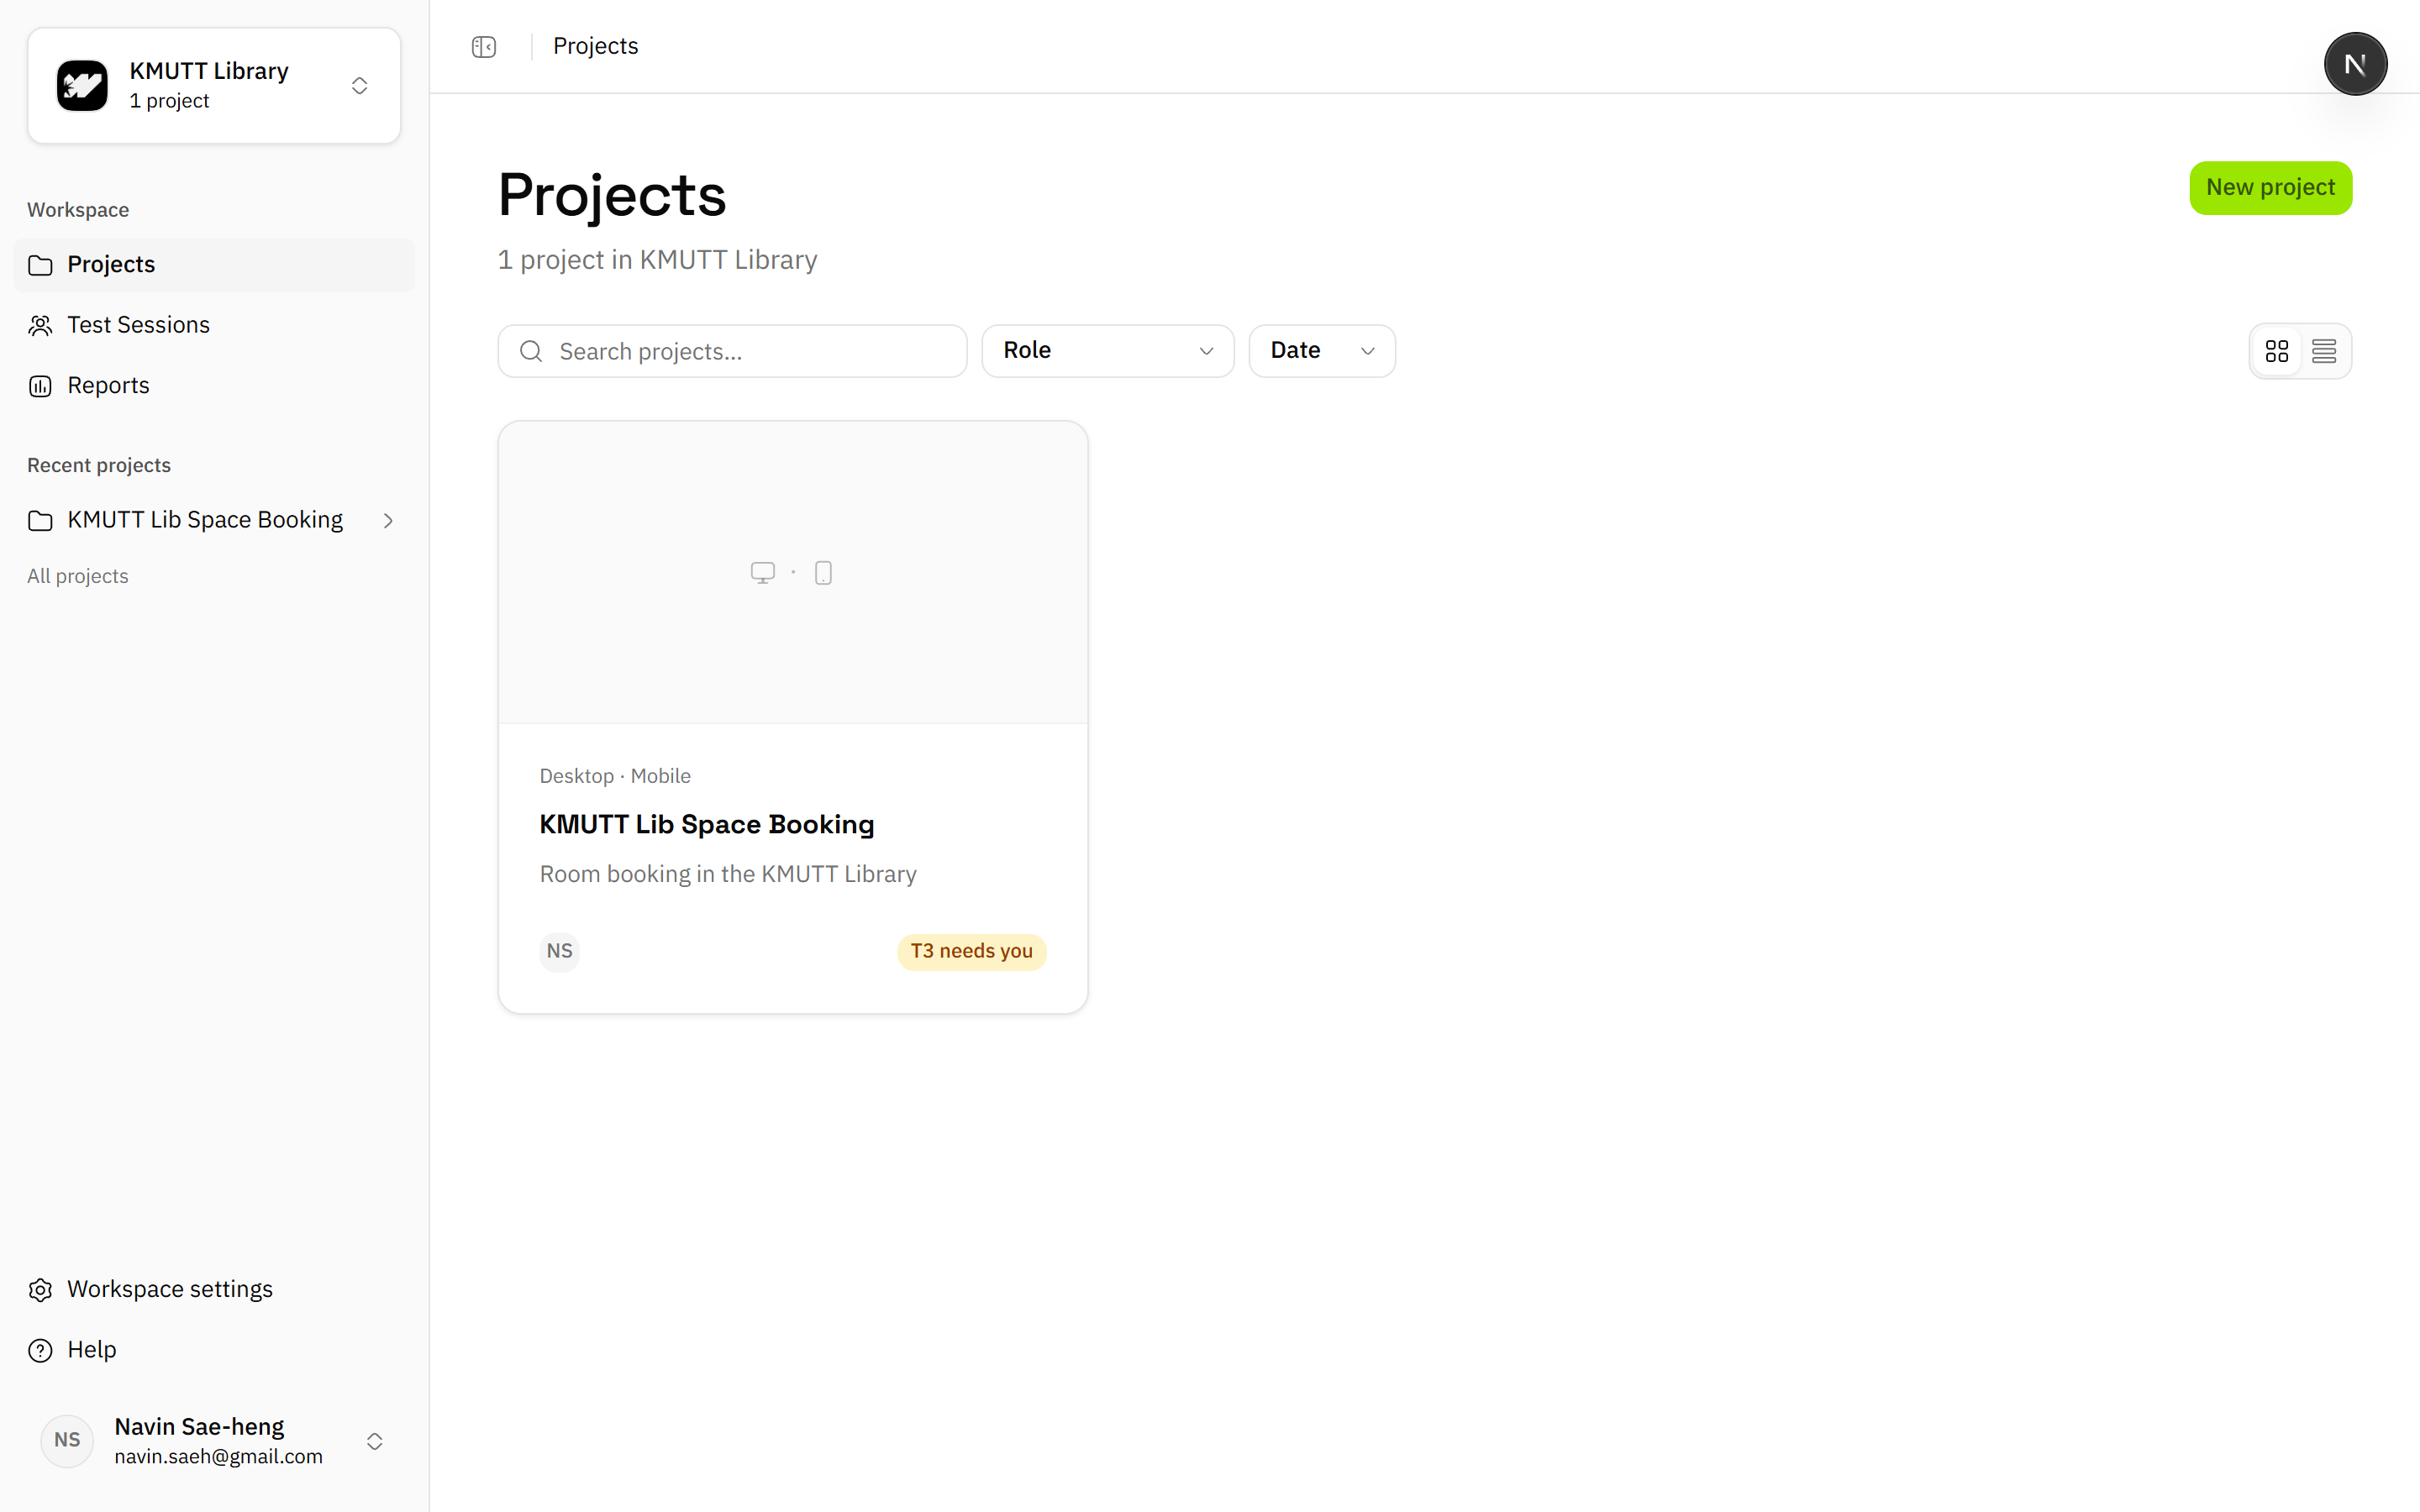
\includegraphics[width=0.9\linewidth]{figures/ch3-methodology/screens/projects.png}
  \caption{หน้ารายการโปรเจกต์ใน workspace}
  \label{fig:screen-projects}
\end{figure}
\begin{figure}[H]
  \centering
  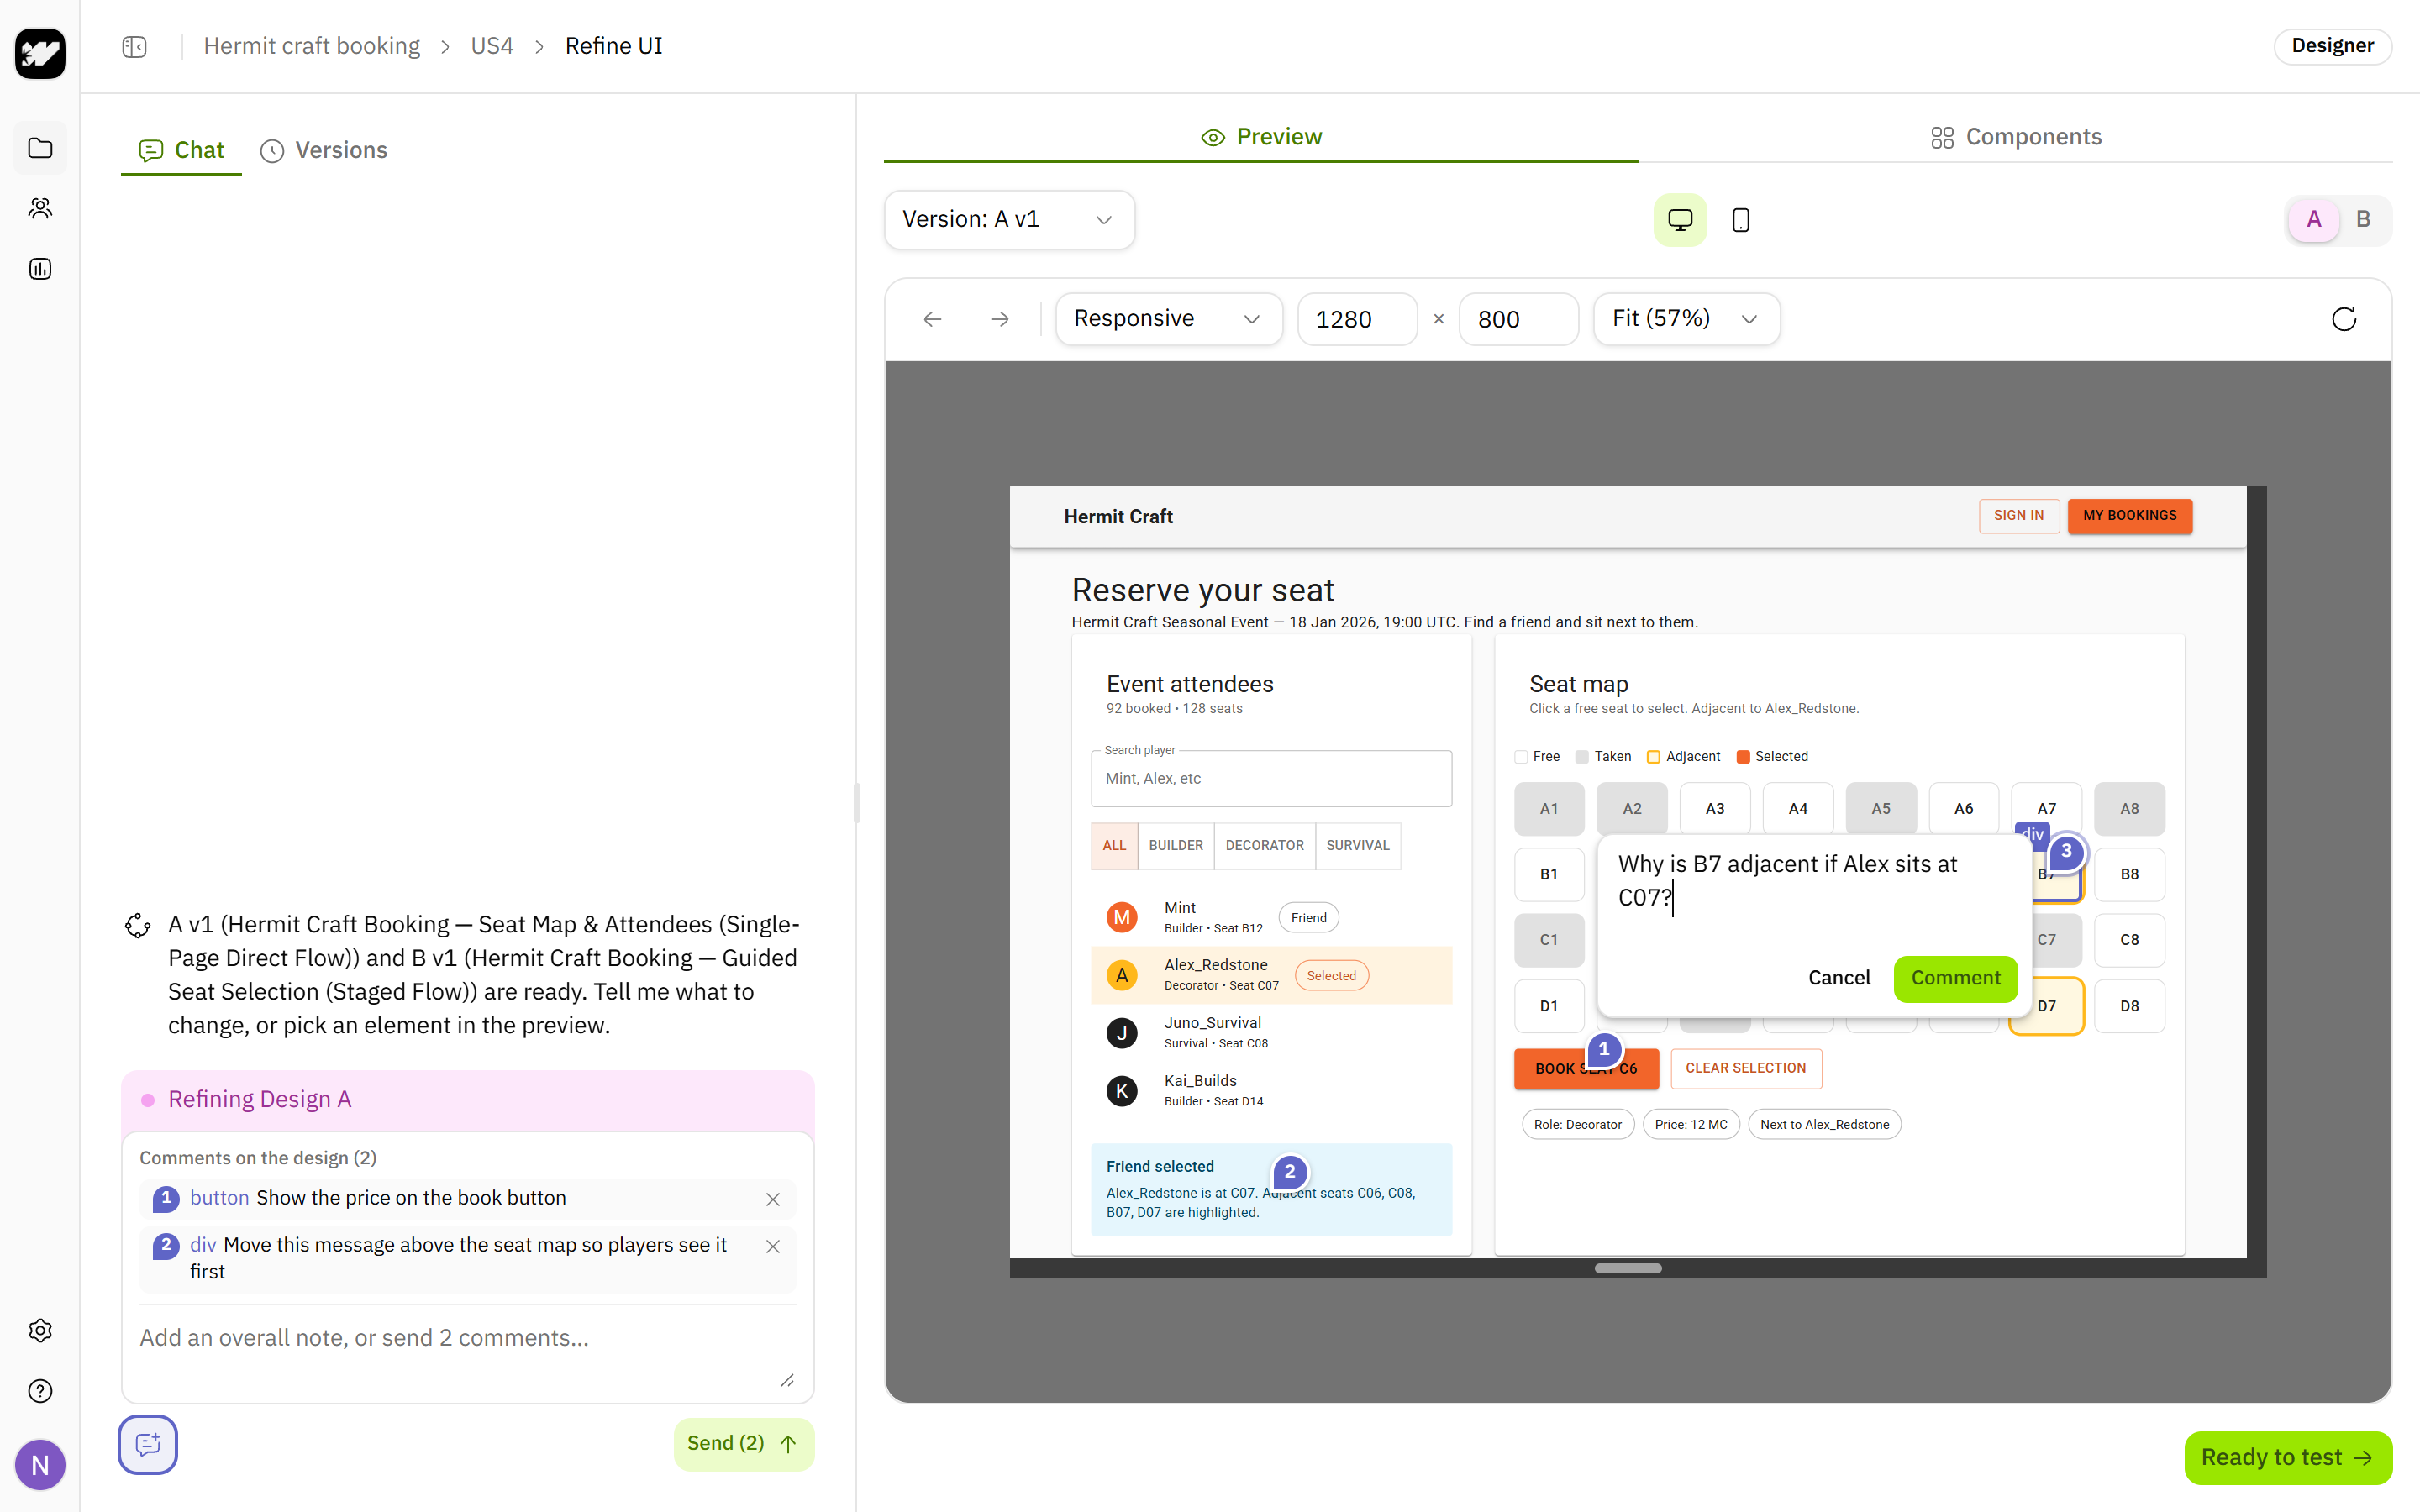
\includegraphics[width=0.9\linewidth]{figures/ch3-methodology/screens/refine-pins.png}
  \caption{หมุดความคิดเห็นบนหน้าตัวอย่างของ variant ในหน้า refine}
  \label{fig:screen-refine-pins}
\end{figure}

\subsection{การพัฒนาหน้าจอเว็บไซต์ของ Usability Tester และผู้มีส่วนได้ส่วนเสีย}
\thaijustify{
  หน้าจอเซสชันการทดสอบ (\texttt{.../sessions}) และรายงาน (\texttt{.../reports}) ปัจจุบันเป็นแท็บในหน้าโปรเจกต์ที่รอเชื่อมกับ API ซึ่ง backend พัฒนาไว้แล้ว (ตารางที่~\ref{tab:api-groups}) หน้าจอของผู้เข้าร่วมทดสอบ และมุมมองของ Client, Developer และ Project Manager อยู่ในแผนของภาคการศึกษาที่ 2
}
